\documentclass[11pt]{article}
\usepackage[margin=1in]{geometry}
\usepackage{graphicx,booktabs,amsmath,hyperref,natbib}
\title{JWST/NIRSpec Micro-Shutter Throughput Loss Sandbox}
\author{Biswajit Jana}
\date{\today}
\begin{document}
\maketitle

\begin{abstract}
This is a bounded, physically-grounded Monte Carlo sandbox exploring how
target-centering error and wavelength-dependent point-spread-function (PSF)
width set a \emph{simplified} geometric slit-loss throughput conditional on
a planned micro-shutter-array (MSA) shutter opening successfully. Static
operability is a target-assignment constraint; random command failure is a
separate sensitivity scenario for JWST/NIRSpec
multi-object spectroscopy. All numeric instrument constants (shutter
geometry, PSF anchor, command-failure boundary, target-acquisition accuracy) are
traced to verified public sources (Jakobsen et al. 2022; Ferruit et al. 2022;
Rawle et al. 2022; NASA JWST spacecraft overview) --- see
Section~\ref{sec:data} and \texttt{data/manifest.csv}. All throughput values
reported here are \textbf{synthetic Monte Carlo output}
(\texttt{data\_kind = "synthetic\_monte\_carlo"}), not real telemetry or an
official pipeline path-loss correction. The forward-model / injection-recovery
validation gate (Section~\ref{sec:validation}) passed. Production-run results
(\texttt{monte\_carlo.production\_trials} trials, Section~\ref{sec:results})
are read directly, unedited, from \texttt{results/summary.json}.
\end{abstract}

\section{Scientific question}
Conditional on a planned shutter opening, how do target-centering error and
wavelength-dependent PSF width alter geometric slit throughput, and what is
the separate penalty under a conservative 0--4\% random non-opening scenario?

\section{Data and provenance}
\label{sec:data}
Per \texttt{docs/DATASET\_PLAN.md}, this project's data mode is
\emph{official instrument parameters + synthetic Monte Carlo}: a
physically-grounded simulation, not an archive-download audit. No real
NIRSpec observational products are downloaded or used. Eight numeric
instrument parameters were verified via \texttt{WebFetch} against real
public sources during the implementation session and are recorded, with
exact source URLs, retrieval timestamps and content hashes, in
\texttt{data/manifest.csv} (mirrored in \texttt{data/provenance.yml}):
shutter pitch and open-aperture dimensions, MSA array layout, historical
operability context, the current random non-opening boundary, NIRSpec wavelength range, the PSF FWHM
anchor at 2.5\,$\mu$m, the JWST primary mirror diameter, and the MSA
target-acquisition accuracy requirement. Two items remain flagged
\texttt{VERIFICATION\_PENDING} rather than fabricated (Section~\ref{sec:limitations}):
the sub-diffraction-limit PSF broadening below 2.46\,$\mu$m, and the spatial
(non-independent) structure of real shutter failures.

\section{Method}
\label{sec:method}
The model treats the NIRSpec PSF as a circularly-symmetric 2-D Gaussian
whose $\sigma(\lambda)$ follows the diffraction-limited $\lambda/D$ scaling
law ($D=6.5$\,m), calibrated to the verified 80\,mas FWHM anchor at
2.5\,$\mu$m (\texttt{psf.py}; reproduces the anchor to $<1\%$ from the pure
geometric law, confirming the correct functional form). For a target whose
PSF centroid is offset by $(dx, dy)$ from a shutter's centre, the
geometrically transmitted flux fraction through the open rectangular
aperture is the exact product of two independent 1-D Gaussian-CDF integrals
(\texttt{geometry.rectangular\_aperture\_transmission}) --- exact given the
Gaussian-PSF assumption, not an additional approximation. Each Monte Carlo
trial draws an independent 2-D centering offset
($\mathcal{N}(0,\sigma_{\mathrm{cent}}^2)$ per axis, fiducial
$\sigma_{\mathrm{cent}}=20$\,mas, the verified MSATA in-flight accuracy), a
wavelength uniform on $[0.6, 5.3]\,\mu$m. Conditional geometric throughput is
estimated only for successful commands. A separate Bernoulli command-success
draw, with failure varied from 0 to 4\%, defines a conservative sensitivity
scenario (\texttt{monte\_carlo.py}); static operability is not multiplied into
throughput because APT/MPT uses position-specific operability in target
assignment. \texttt{core.run\_pipeline} composes the trial
ensemble with two deterministic diagnostic sweeps (throughput vs.\ offset at
fixed wavelength; throughput vs.\ wavelength at fixed offset) and an
illustrative command-success heatmap for the declared scenario.

\emph{Scope note}: this models only the geometric slit-loss component of
throughput --- not detector quantum efficiency, optical-train reflectivity or
grating efficiency --- consistent with the bounded ``simplified'' scientific
question (\texttt{docs/RESEARCH\_BLUEPRINT.md}).

\section{Validation and uncertainty}
\label{sec:validation}
Monte Carlo placement/observational uncertainty is reported via bootstrap
resampling of the per-trial throughput ensemble (1000 resamples, 95\%
confidence, seed 20260713, \texttt{uncertainty.bootstrap\_statistic});
numerical fit convergence (used only when fitting an effective centering
sigma back out of a throughput-vs-offset sweep) is assessed separately via
covariance condition number and reduced $\chi^2$
(\texttt{uncertainty.check\_fit\_convergence}) --- the two uncertainty
categories are never conflated.

\textbf{Analytic-limit validation}
(\texttt{tests/test\_geometry.py::test\_transmission\_matches\_analytic\_zero\_offset\_closed\_form}):
at zero offset, the general numerical transmission function agrees with the
independently-derived closed-form $\mathrm{erf}$ expression to $<10^{-9}$
relative precision. \textbf{Injection recovery}
(\texttt{tests/test\_core\_pipeline.py::test\_injection\_recovery\_effective\_sigma}):
a known effective 1-D PSF sigma (55\,mas) is injected into the noise-free
forward model across a 40-point offset sweep and fit back out via
\texttt{core.recover\_effective\_sigma} (fit parameter normalized to $O(1)$
before fitting); the recovered value matches the injected truth to
$<0.1\%$ relative error, and the fit's covariance conditioning passes.
\textbf{This gate passed.} \textbf{Null control}
(\texttt{tests/test\_throughput.py::test\_null\_control\_zero\_offset\_all\_open\_large\_aperture\_near\_unity}):
zero centering error, all shutters operable, and an aperture much larger than
the PSF together drive throughput to $1.0$ within $10^{-6}$.
\textbf{Failure modes}: zero Monte Carlo trials raises
\texttt{InsufficientDataError} rather than returning a degenerate result
(\texttt{test\_run\_pipeline\_rejects\_zero\_trials}); non-finite or
out-of-shape trial inputs raise \texttt{DataSchemaError}; an ill-conditioned
or non-finite fit covariance raises \texttt{ConvergenceError}.

\section{Results}
\label{sec:results}
All numbers below are read directly, unedited, from
\texttt{results/summary.json}, produced by \texttt{scripts/run\_analysis.py}
at the production trial count configured in
\texttt{config/analysis.yml} (\texttt{monte\_carlo.production\_trials} =
20{,}000 trials).

Averaged over successful-command trials ($n=19{,}178$ in the seeded
20{,}000-trial run), the mean conditional geometric throughput is $0.9490$
(95\% bootstrap interval $[0.9482, 0.9499]$), with median $0.9777$. Under the
separate 4\% random non-opening scenario, the realised failure fraction is
$0.0411$ and the mean effective scenario throughput is $0.9100$. The former
$0.7795$ headline is retired because it multiplied conditional transmission
by an aggregate planning-operability fraction as though every statically
unavailable shutter were an independent photon-loss event. The
offset sweep (Figure~\ref{fig:offset}) shows the expected smooth,
symmetric roll-off: throughput exceeds $0.98$ within $\pm 15$\,mas of
perfect centering and falls to $\sim\!0.10$ by $\pm 150$\,mas, consistent
with the verified $\sim\!20$\,mas MSATA accuracy being small relative to
the $\sim\!268$\,mas shutter pitch. The wavelength sweep
(Figure~\ref{fig:wavelength}) shows throughput near unity shortward of the
verified $2.46\,\mu$m diffraction-limit onset, declining smoothly to
$\sim\!0.82$ at the $5.3\,\mu$m red edge of the NIRSpec range as the
diffraction-limited PSF broadens --- the qualitative direction expected from
the $\lambda/D$ scaling law, though the true short-wavelength values are
likely somewhat more optimistic than reality per the PSF-broadening
limitation below.

\section{Limitations}
\label{sec:limitations}
An instrument-physics QA sandbox; not a replacement for the JWST pipeline or
official path-loss corrections. The PSF is modelled as a circularly-symmetric
2-D Gaussian, not the true NIRSpec Airy/diffraction pattern with wings. The
pure diffraction-limited $\lambda/D$ PSF scaling is applied across the full
0.6--5.3\,$\mu$m NIRSpec range, though the literature anchor only confirms
Strehl$>0.8$ above 2.46\,$\mu$m --- below that, the true PSF is likely
somewhat broader than modelled here, so short-wavelength slit losses are
likely somewhat \emph{underestimated} (\texttt{VERIFICATION\_PENDING}, no verified
quantitative Strehl-vs-wavelength curve was found in the time available).
Static shutter operability is position-specific planning information and is
excluded from the throughput estimator. The 0--4\% random non-opening term is
an independent sensitivity boundary, not a target-specific prediction; the
real spatial and temporal failure structure is not reproduced. Field-averaged shutter pitch/open-area
values are used; true values vary $\sim$1--4\% across the field of view due
to optical distortion (not modelled). See
\texttt{docs/ASSUMPTIONS\_AND\_LIMITATIONS.md} for the full list.

\section{Reproducibility}
\begin{verbatim}
python -m pip install -e ".[dev]"
pytest -q
ruff check src tests scripts
mypy src
python scripts/fetch_data.py --i-have-authorization   # verifies data/manifest.csv only, no network I/O
python scripts/run_analysis.py --demo                 # small trial count
python scripts/run_analysis.py                        # full production trial count
python scripts/make_figures.py --demo
python scripts/make_figures.py
python scripts/sync_web_assets.py
\end{verbatim}
Software version, git commit and configuration SHA-256 are recorded in
\texttt{results/summary.json} and each figure's sidecar JSON.

\begin{figure}
  \centering
  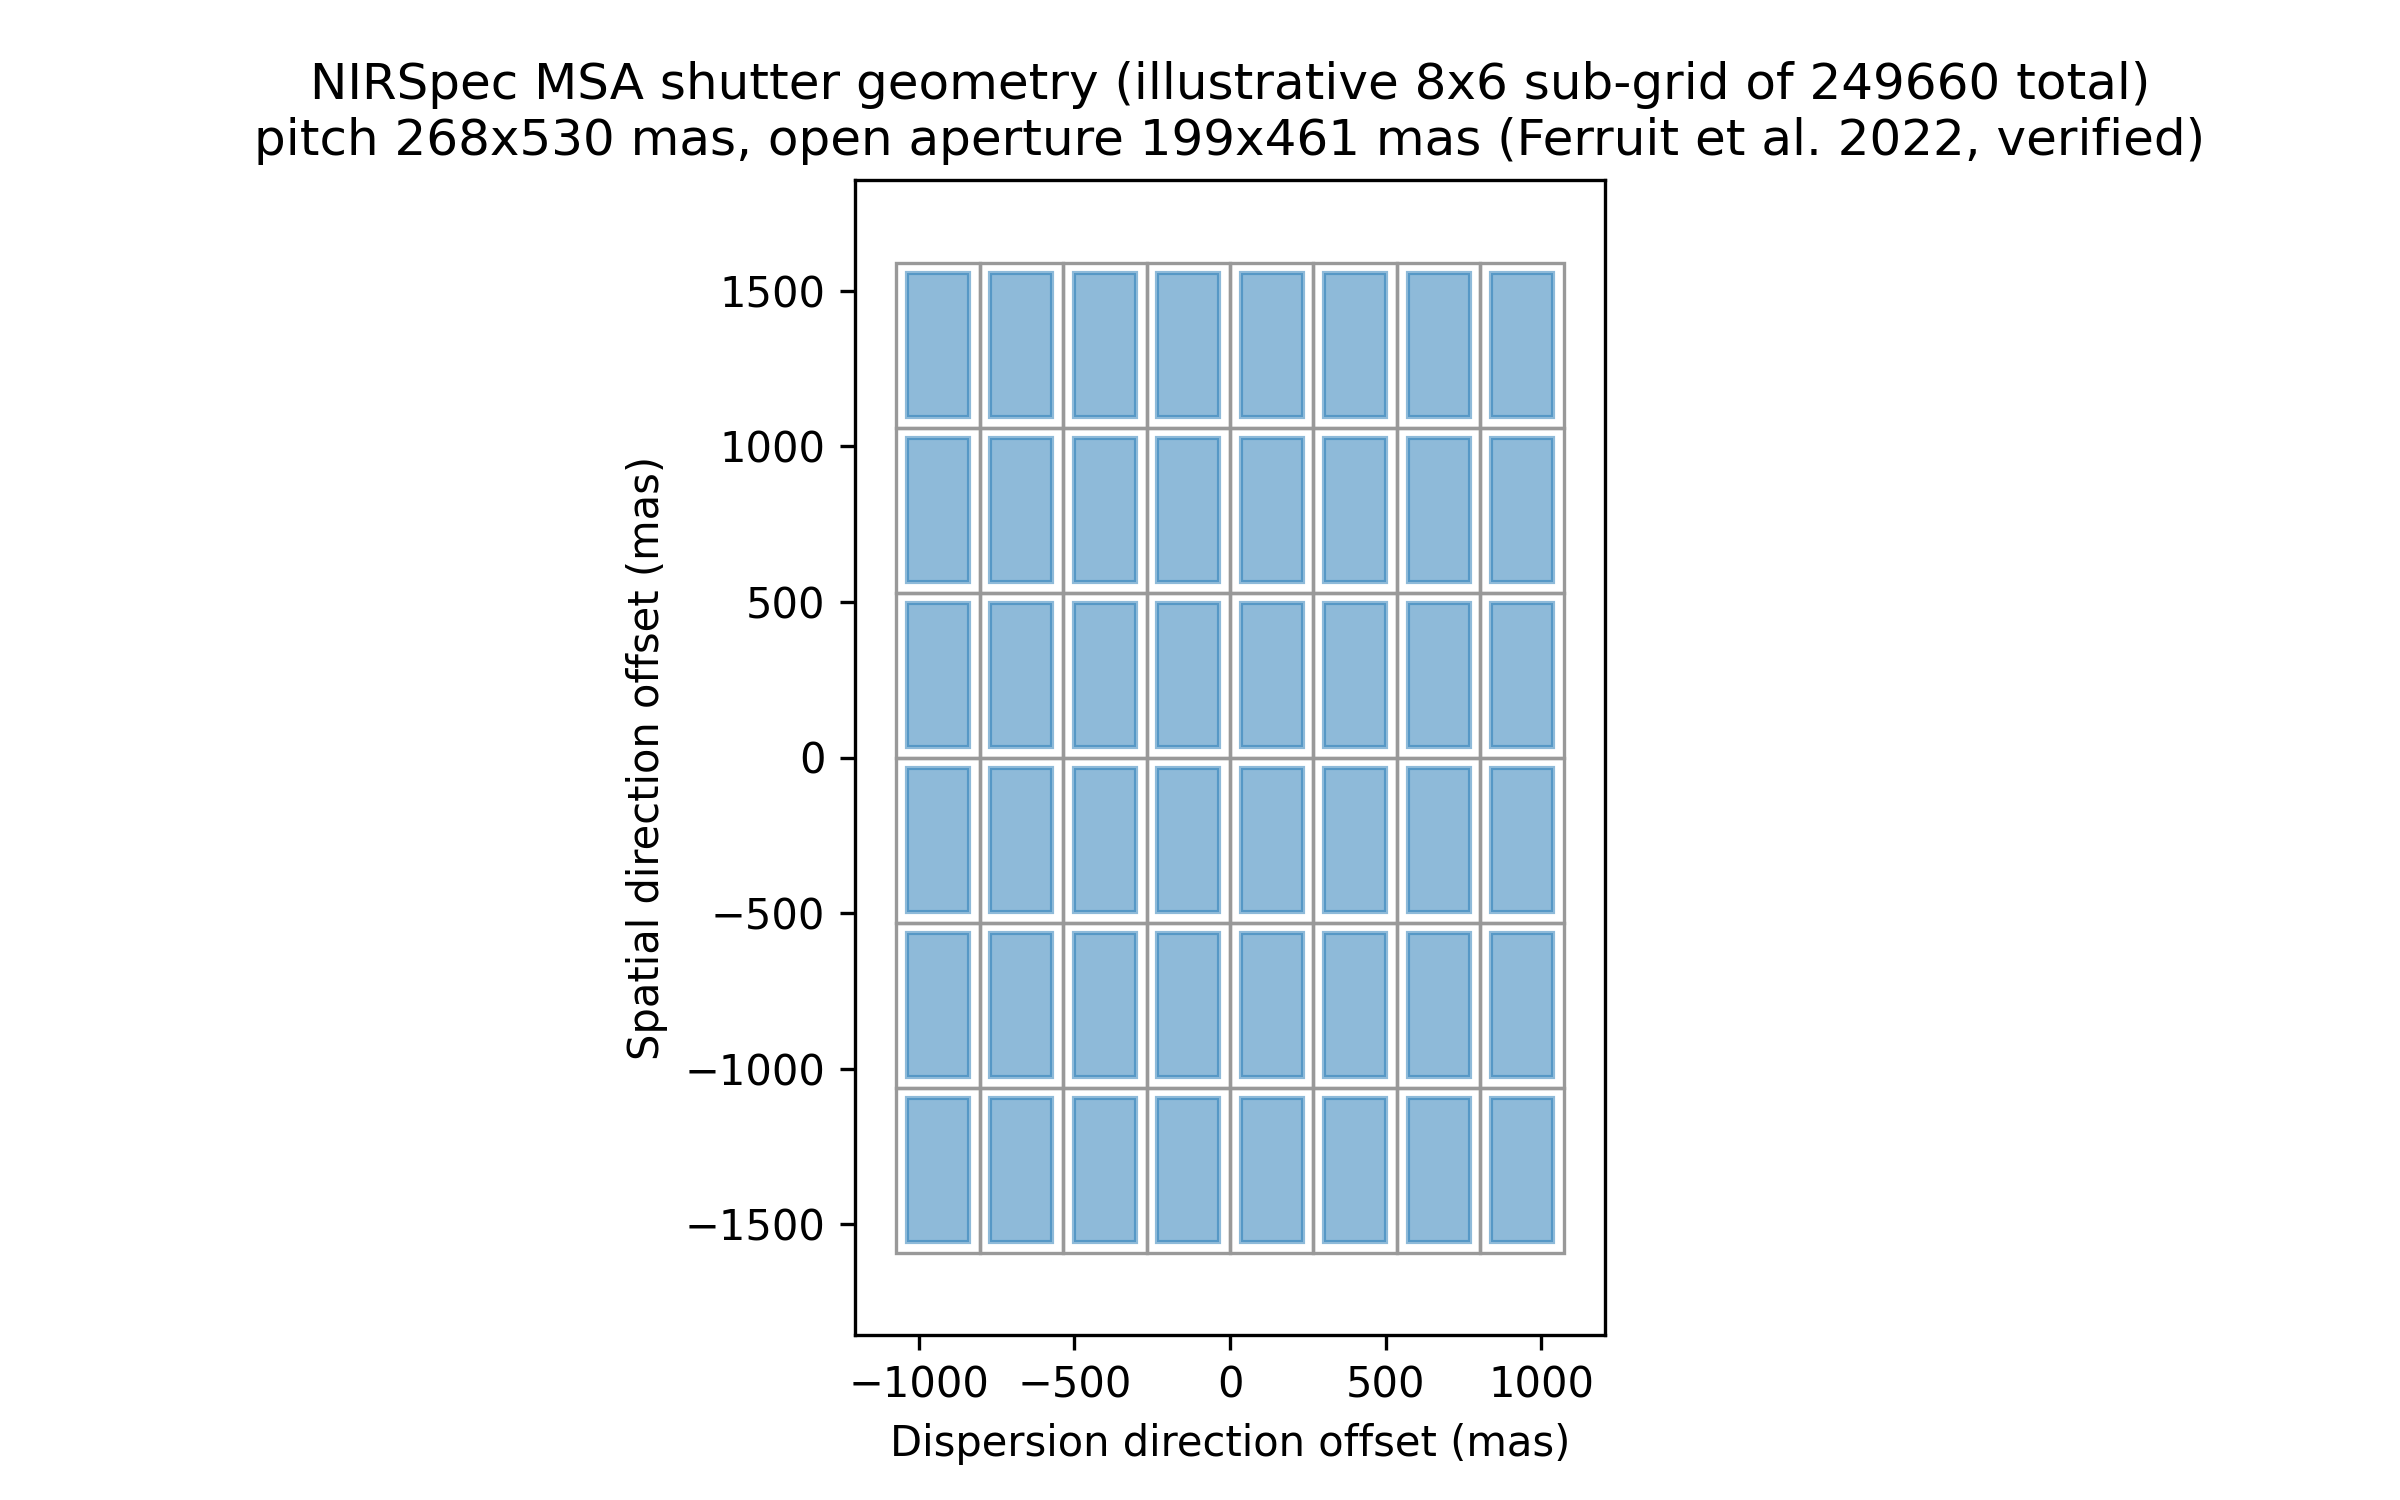
\includegraphics[width=0.7\textwidth]{../figures/fig01_msa_geometry.png}
  \caption{NIRSpec MSA shutter geometry: illustrative sub-grid with verified
  pitch and open-aperture dimensions annotated (Ferruit et al. 2022).}
  \label{fig:geometry}
\end{figure}

\begin{figure}
  \centering
  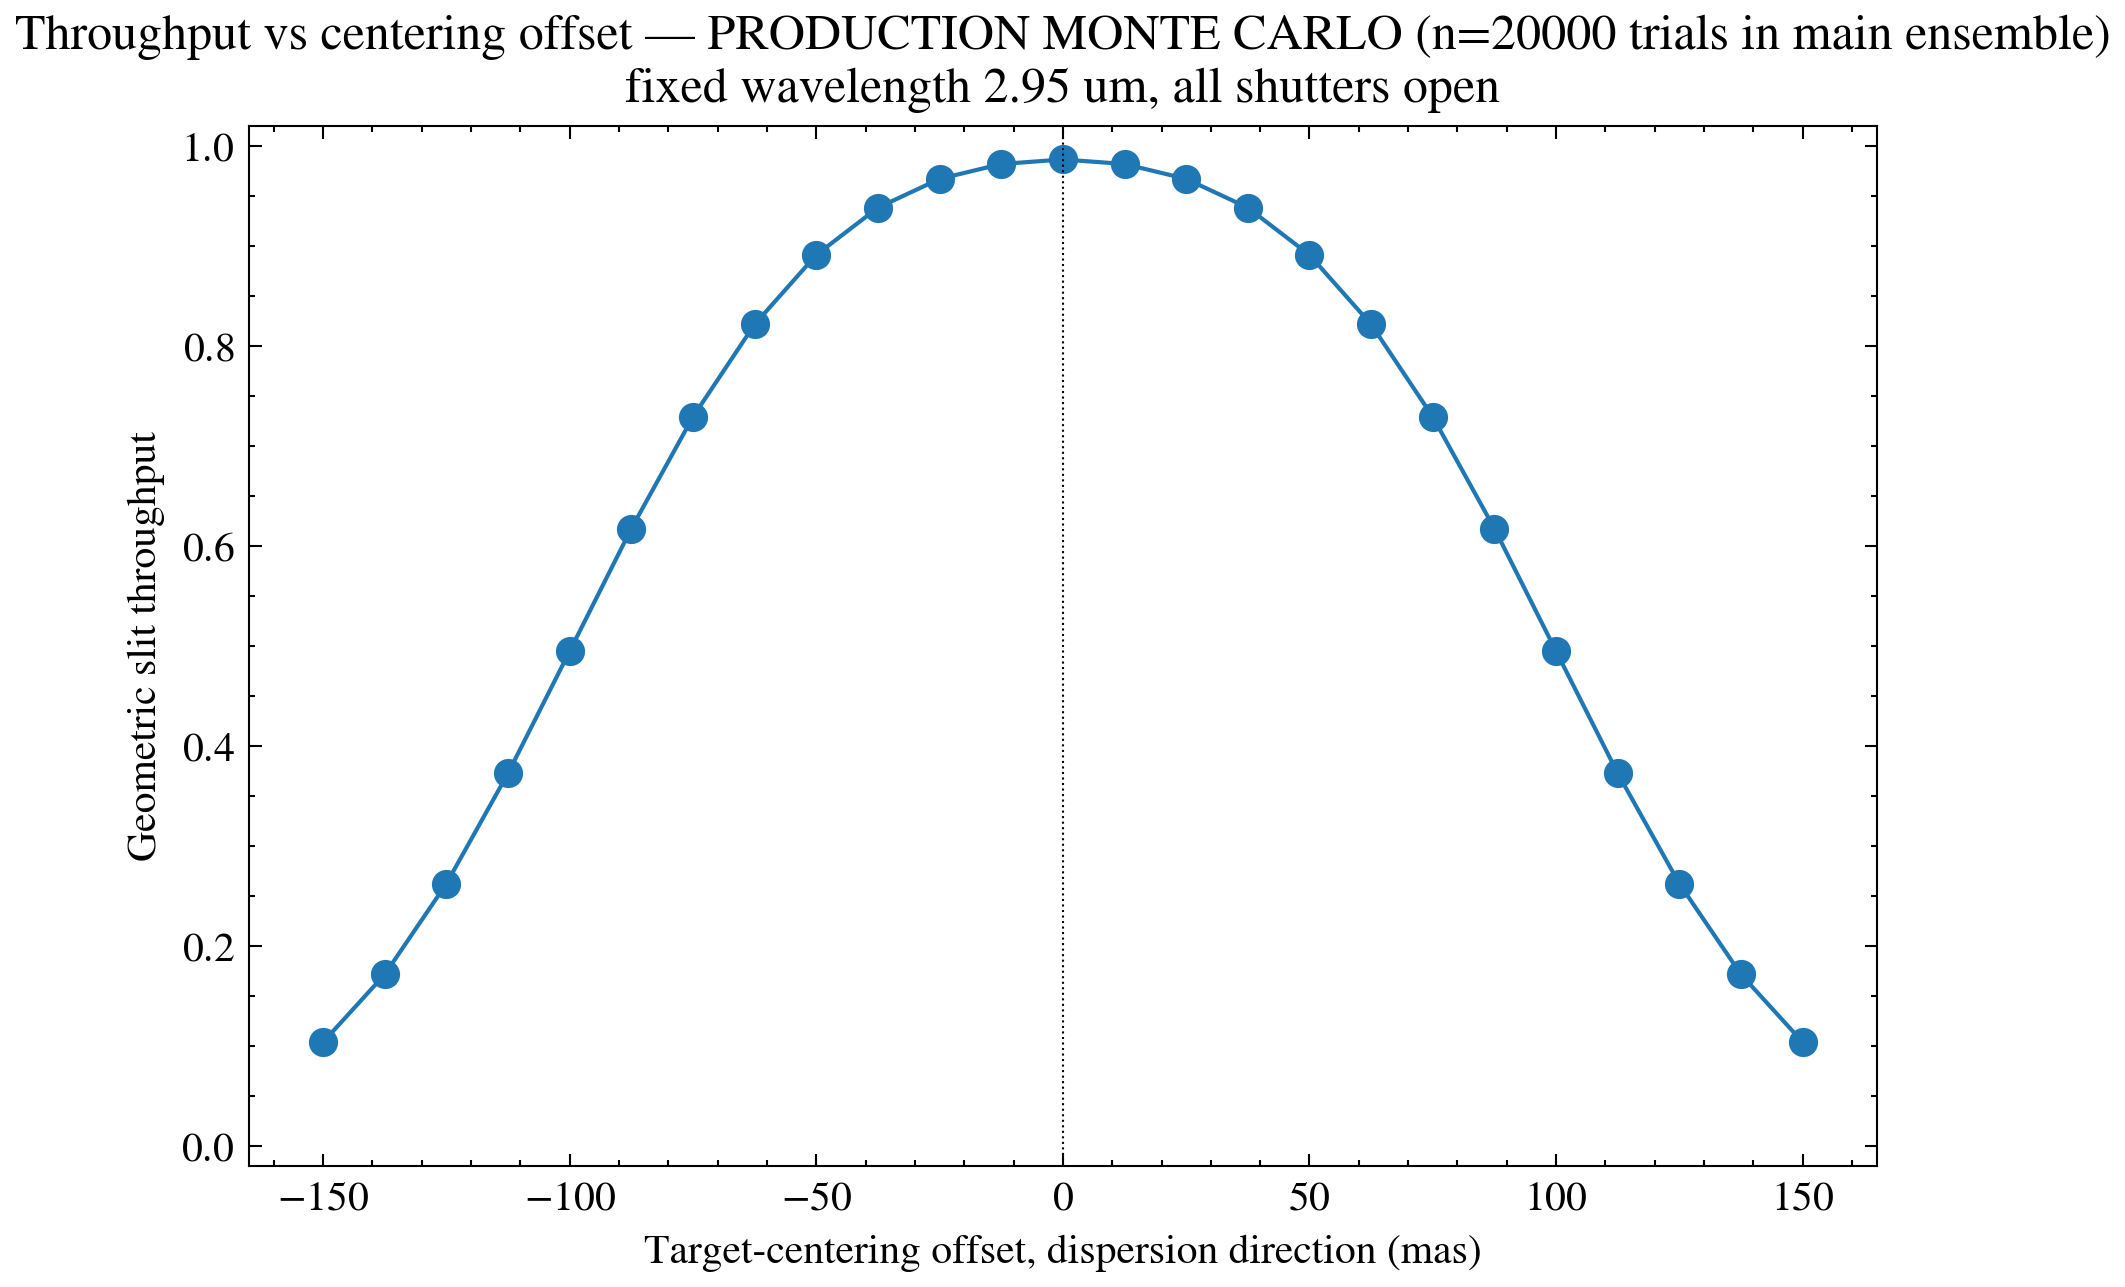
\includegraphics[width=0.7\textwidth]{../figures/fig02_throughput_vs_offset.png}
  \caption{Geometric slit throughput vs.\ target-centering offset (dispersion
  direction), fixed fiducial wavelength, all shutters open.}
  \label{fig:offset}
\end{figure}

\begin{figure}
  \centering
  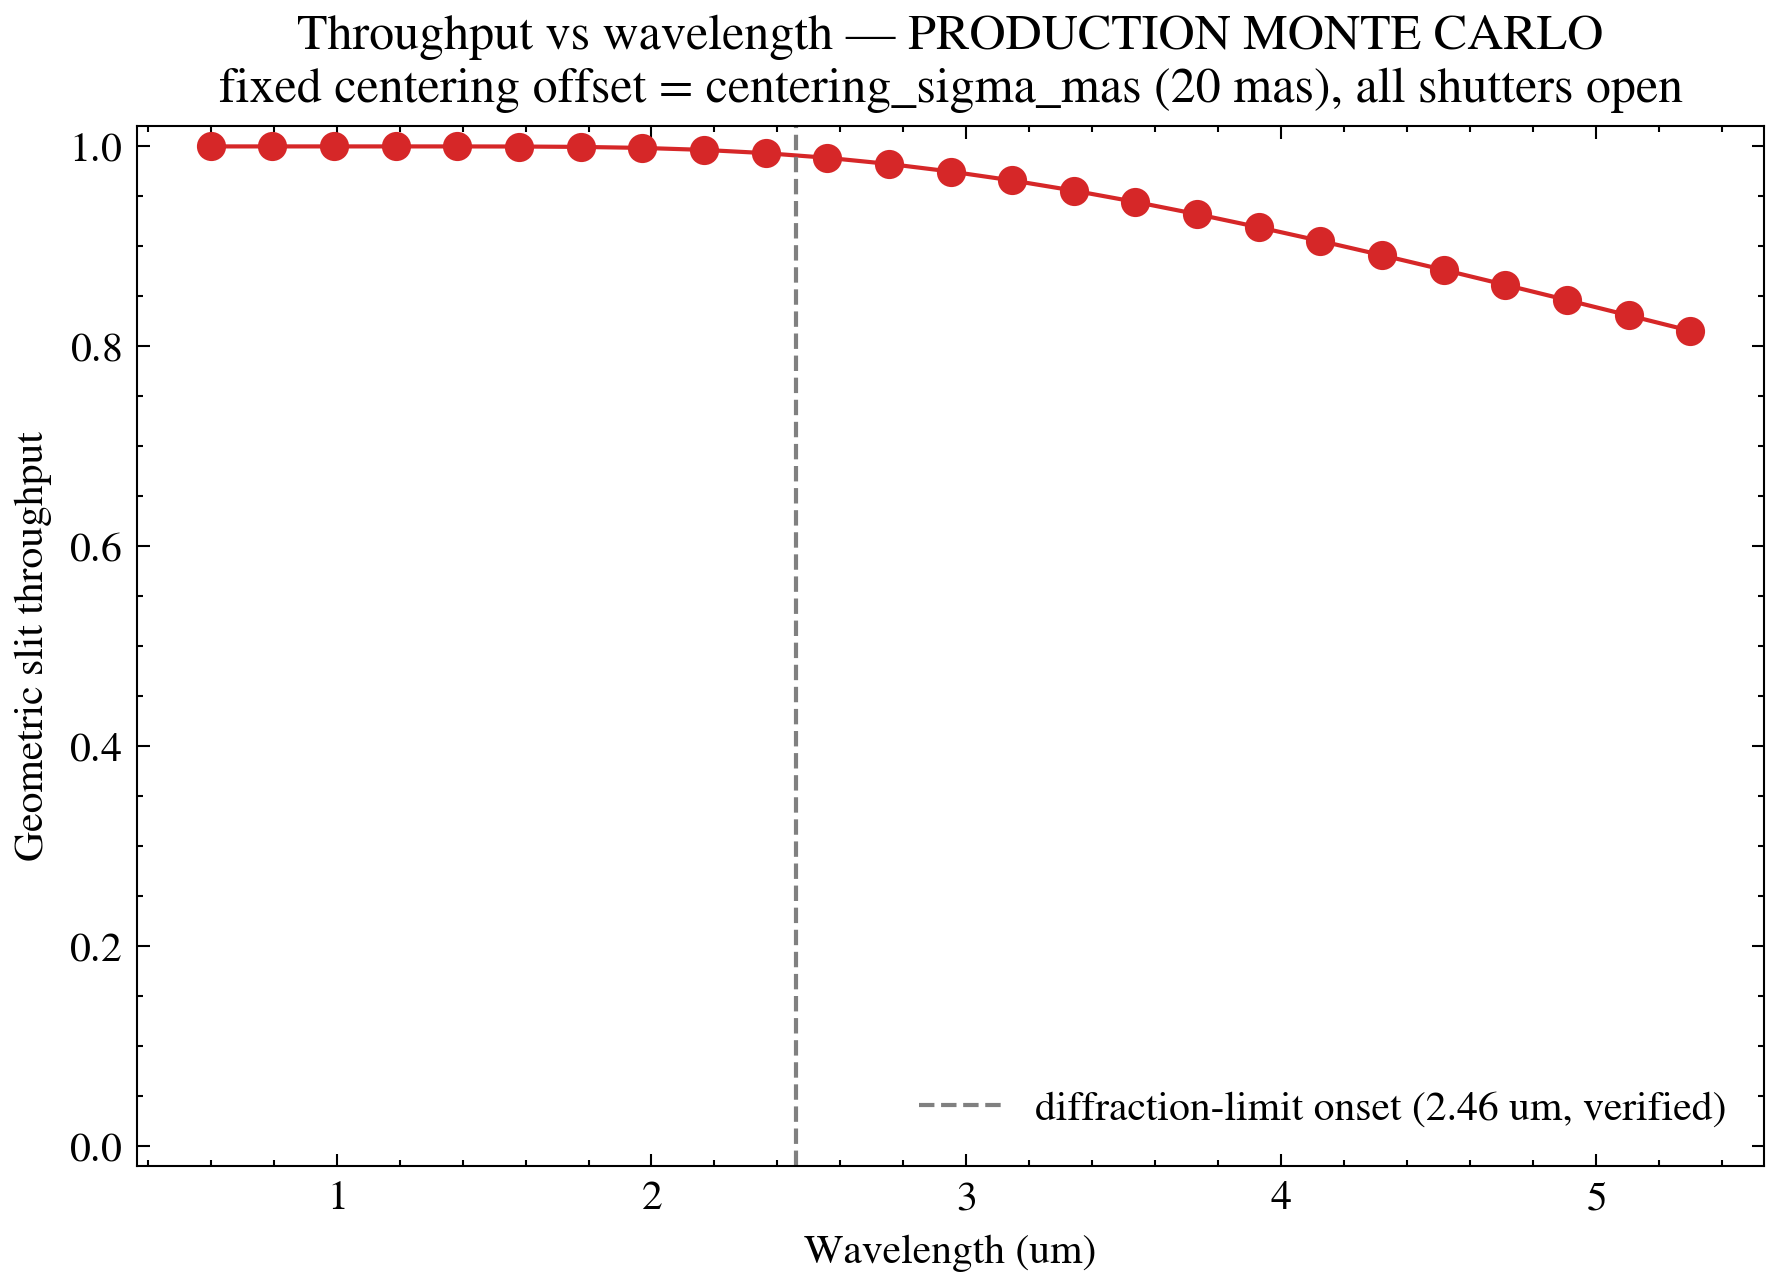
\includegraphics[width=0.7\textwidth]{../figures/fig03_wavelength_loss.png}
  \caption{Geometric slit throughput vs.\ wavelength at the fiducial
  centering-error sigma, all shutters open. Diffraction-limit onset
  (2.46\,$\mu$m, verified) marked.}
  \label{fig:wavelength}
\end{figure}

\begin{figure}
  \centering
  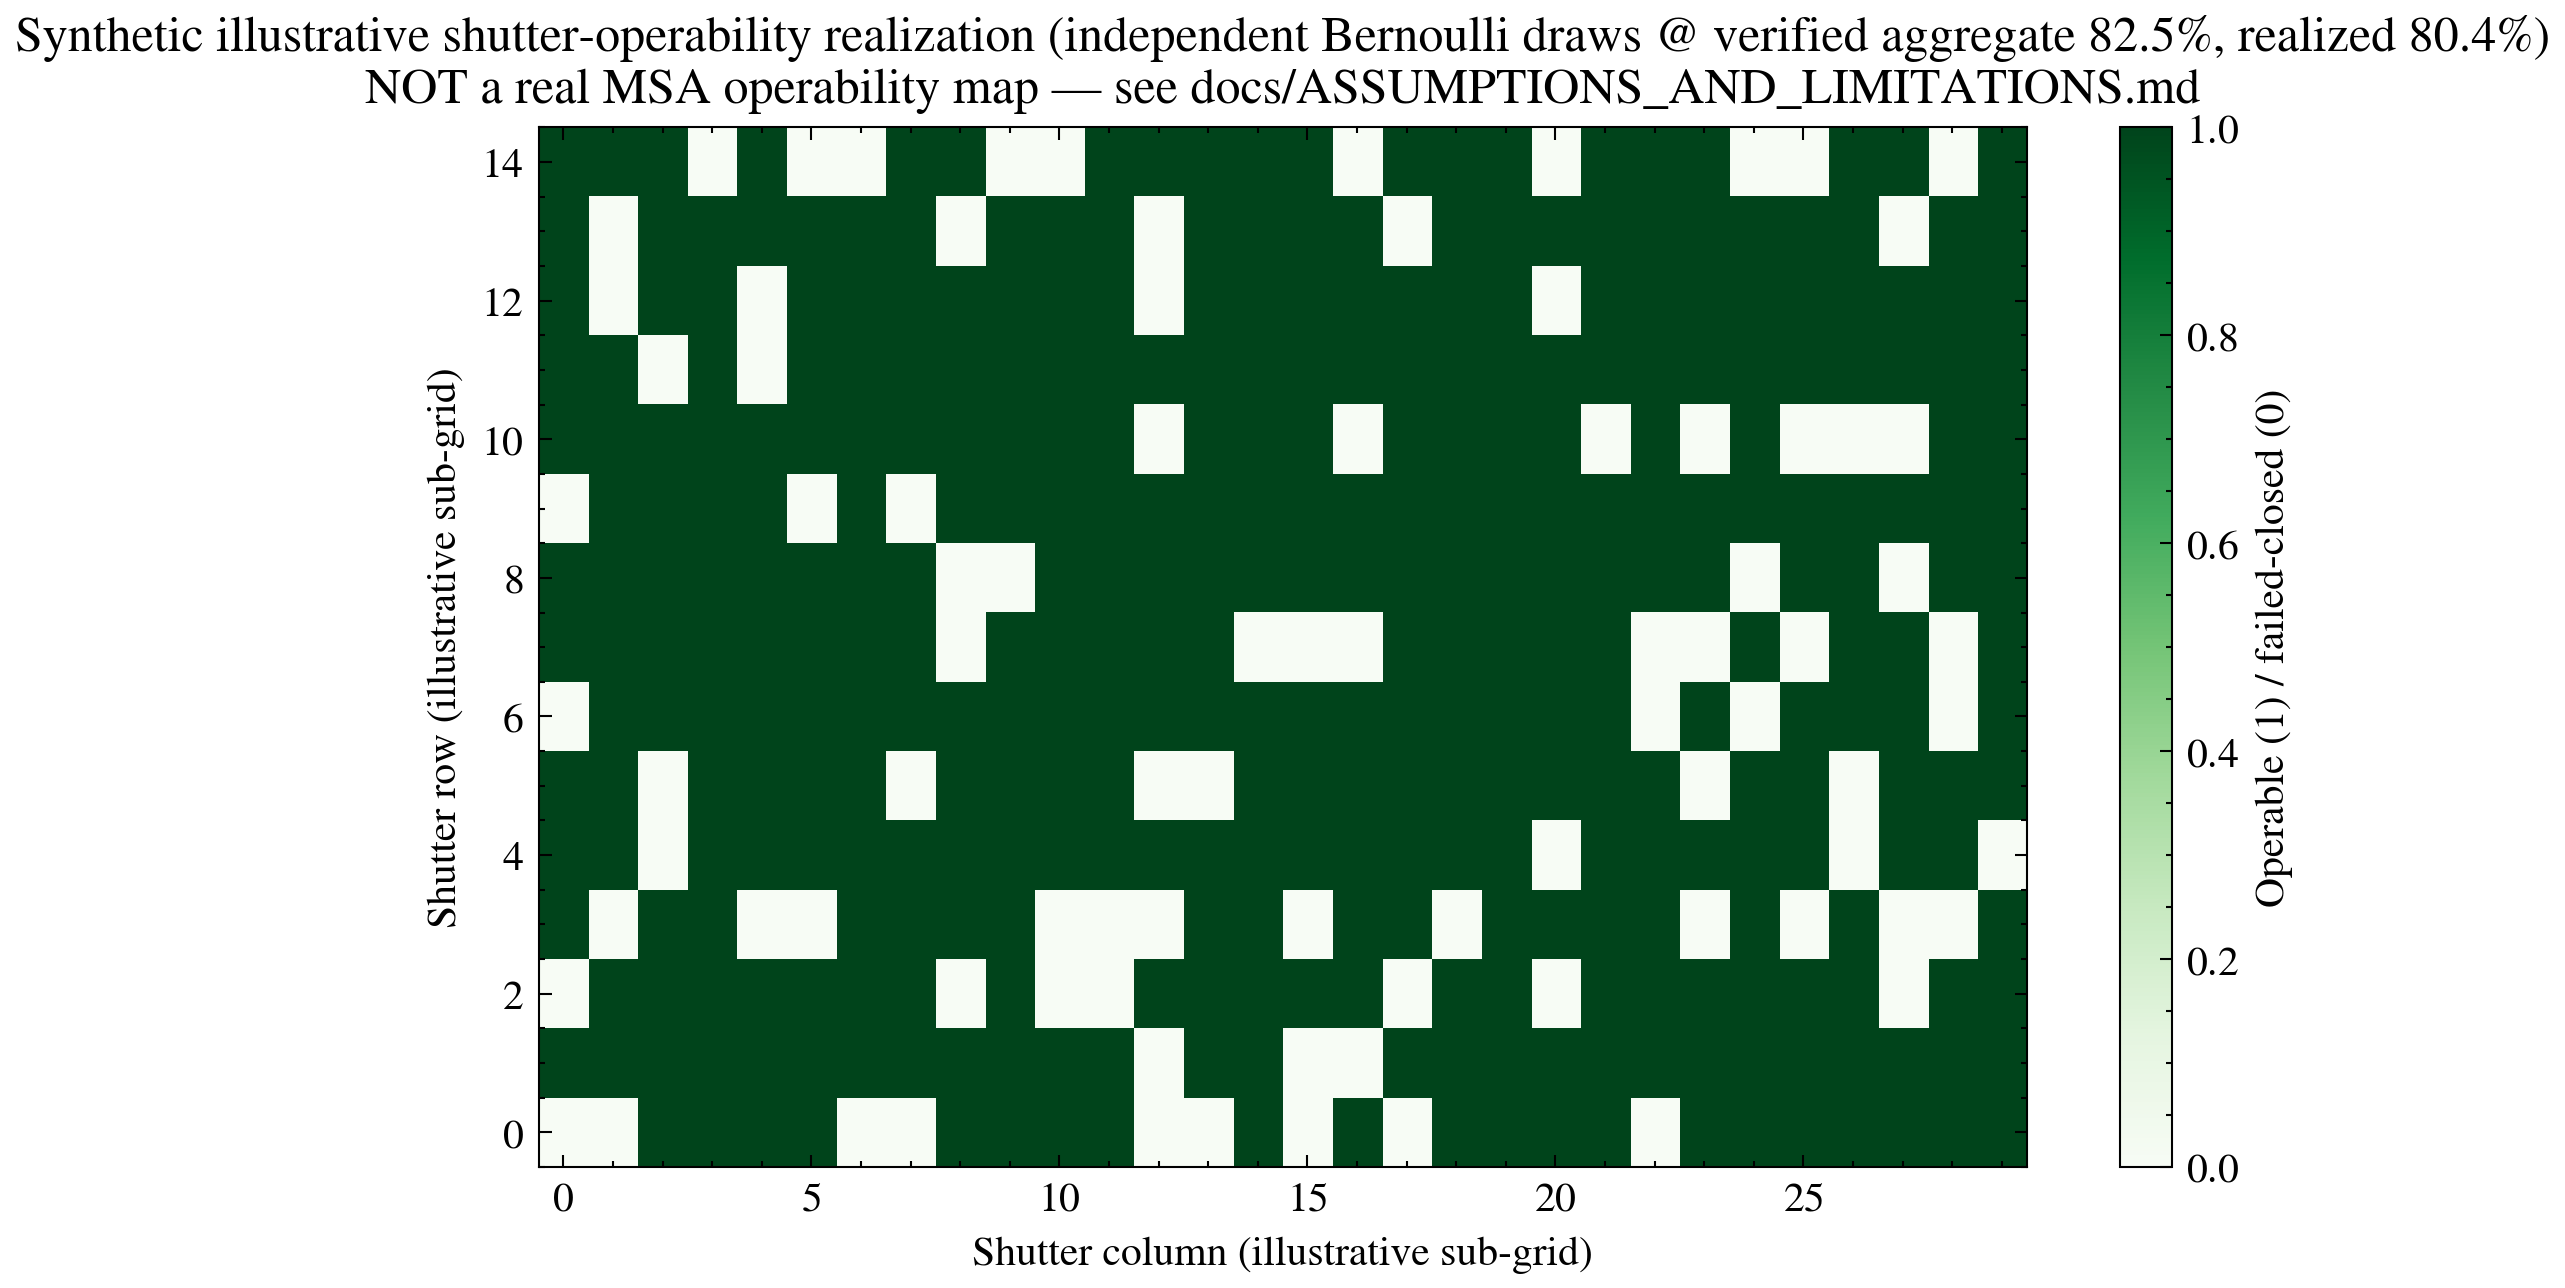
\includegraphics[width=0.7\textwidth]{../figures/fig04_failed_shutter_heatmap.png}
  \caption{Synthetic illustrative command-success realization for the
  conservative 4\% random non-opening scenario --- \textbf{not} a real MSA
  operability map or a target-specific forecast.}
  \label{fig:heatmap}
\end{figure}

\bibliographystyle{plain}
\bibliography{references}
\end{document}
